\apendice{Documentación de usuario}

\section{Introducción}
En este anexo se va a realizar un manual de usuario detallado en el que se describa el uso de las diferentes características que ofrece el \textit{software} desarrollado de una forma sencilla para que cualquier persona sea capaz de entenderlo y poder utilizar la aplicación con normalidad, reduciendo la curva de aprendizaje que habría si no se tuviese este manual.

\section{Requisitos de usuarios}
Al tratarse de una aplicación web, los requisitos necesitados no son demasiados.
El usuario final de la aplicación tan solo necesita contar con un dispositivo con acceso a internet (en caso de tener la aplicación desplegada en un servidor externo a la red del dispositivo) y un navegador web con JavaScript habilitado.

El \textit{software} desarrollado cuenta con un correcto funcionamiento, al menos, bajo cualquiera de los siguientes navegadores:

\begin{enumerate}
\item Google Chrome (probado bajo la versión 114.0.5735.135)
\item Mozilla Firefox (probado en la versión 114.0.2)
\item Microsoft Edge (probado en la versión 114.0.1823.58)
\item Safari
\item Opera (probado en la versión 100.0.4815.21)
\end{enumerate}

\section{Instalación}
Al tratarse de una aplicación web no precisa de instalación, tan solo se debe acceder a la URL bajo la que se encuentre desplegada la aplicación. 
A la hora de realizar este trabajo, la URL de acceso es \url{https://flask-ubu.herokuapp.com/}

\section{Manual del usuario}
El siguiente manual de usuario se va a realizar con un usuario con permisos de modificación para poder mostrar todas las características de la web.
En caso de contar con un usuario con únicamente permisos de lectura, se mostrará parte de la información que aparece en este manual y otros elementos se encontrarán ocultos.

\subsection{Inicio de sesión}

Para comenzar a utilizar la aplicación lo primero que se debe hacer es acceder a la URL\footnote{A día de realización del trabajo: \url{https://flask-ubu.herokuapp.com/}} de la aplicación.

Al acceder a la dirección de la web por primera vez, se mostrará la página de inicio de sesión (ver figura~\ref{pag:login}) desde donde se debe indica el correo electrónico y la contraseña de la cuenta a utilizar.
La cuenta de correo y la contraseña debe ser la misma que la utilizada en el Moodle de la universidad.

\begin{figure}
	\centering
	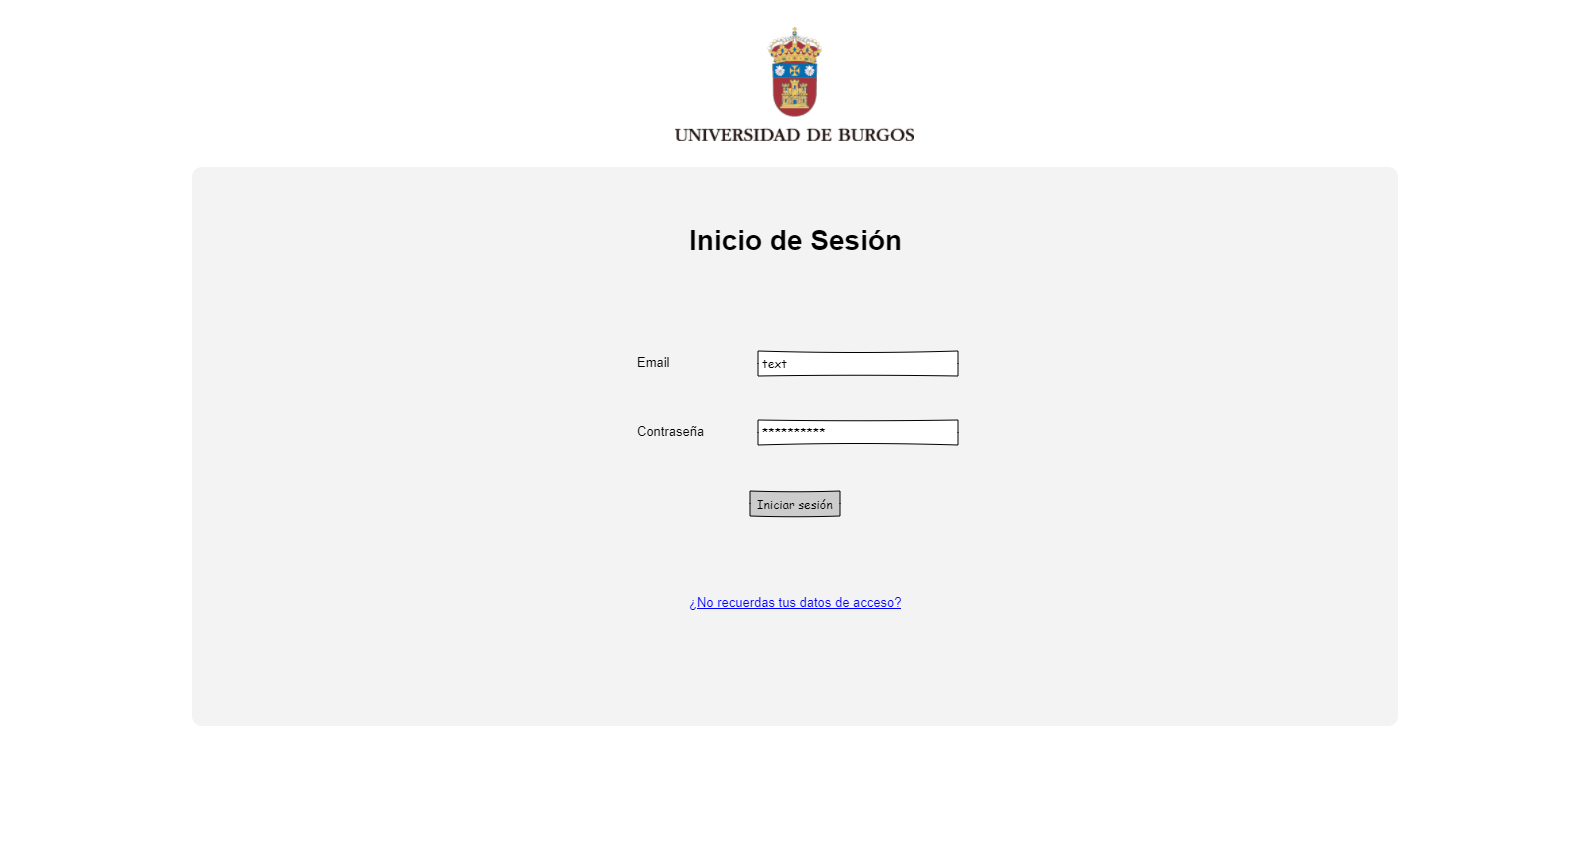
\includegraphics[width=\textwidth]{../img/Anexos/Manual usuario/login.png}
	\caption{Página de inicio de sesión}\label{pag:login}
\end{figure}

Si los datos de acceso son correctos, se tendrá acceso a la aplicación y se mostrará la página principal (imagen~\ref{pag:inicio}).
Una vez se tiene acceso a esta página, se puede acceder al resto de recursos de la web a través del menú superior de navegación.

\begin{figure}
	\centering
	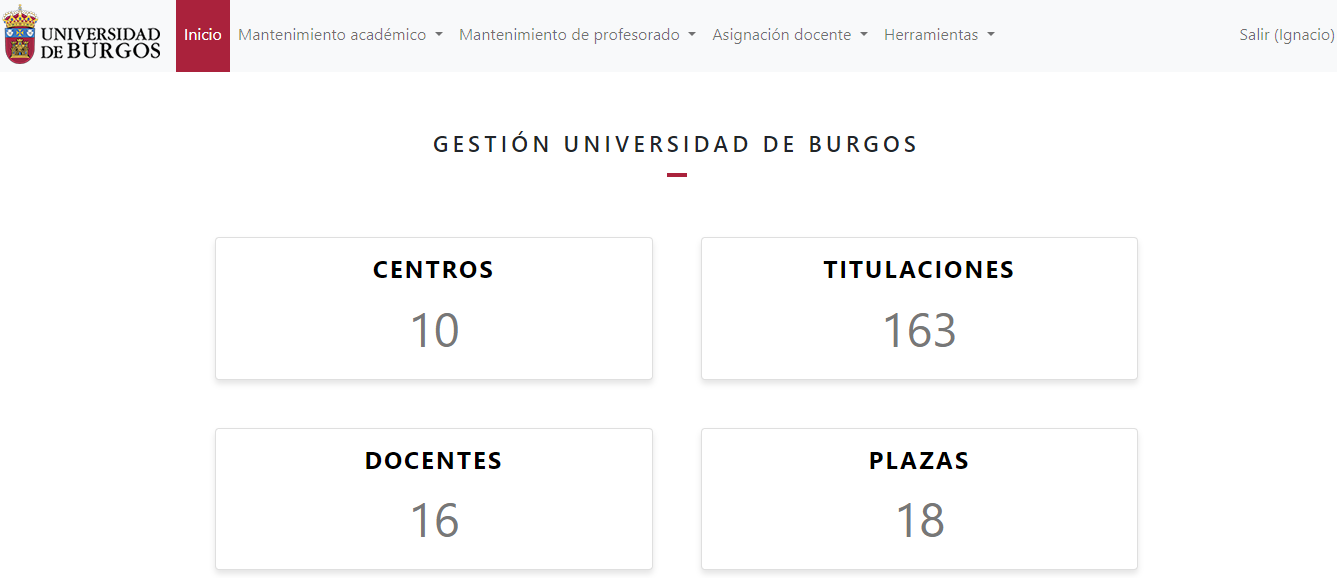
\includegraphics[width=\textwidth]{../img/Anexos/Manual usuario/inicio.png}
	\caption{Página principal}\label{pag:inicio}
\end{figure}

\subsection{Mantenimiento académico}
A continuación se van mostrar las diferentes funcionalidades dentro del mantenimiento académico de la aplicación.
Para ello, se debe pulsar sobre la opción del menú llamada <<Mantenimiento académico>> desde la que se desplegarán las opciones disponibles dentro de esta (imagen~\ref{pag:menuManAc}), las cuales son <<Centros>>, <<Titulaciones>> y <<Asignaturas>>.
Desde cada una de estas opciones se podrá realizar la visualización, creación y actualización de cada uno de estos componentes.

\begin{figure}
	\centering
	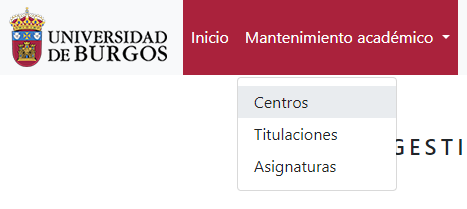
\includegraphics[width=\textwidth]{../img/Anexos/Manual usuario/menu man ac.png}
	\caption{Menú: Mantenimiento académico}\label{pag:menuManAc}
\end{figure}

\subsubsection{Creación de centros}
Pulsando sobre la opción del menú <<Centros>> se accede a la vista principal de los centros de la aplicación (imagen~\ref{pag:centros}).
Para crear un nuevo centro se debe pulsar sobre el botón <<Nuevo>> lo que provocará una redirección a la página que contiene el formulario de creación de centros (imagen~\ref{pag:formCentro}).

\begin{figure}
	\centering
	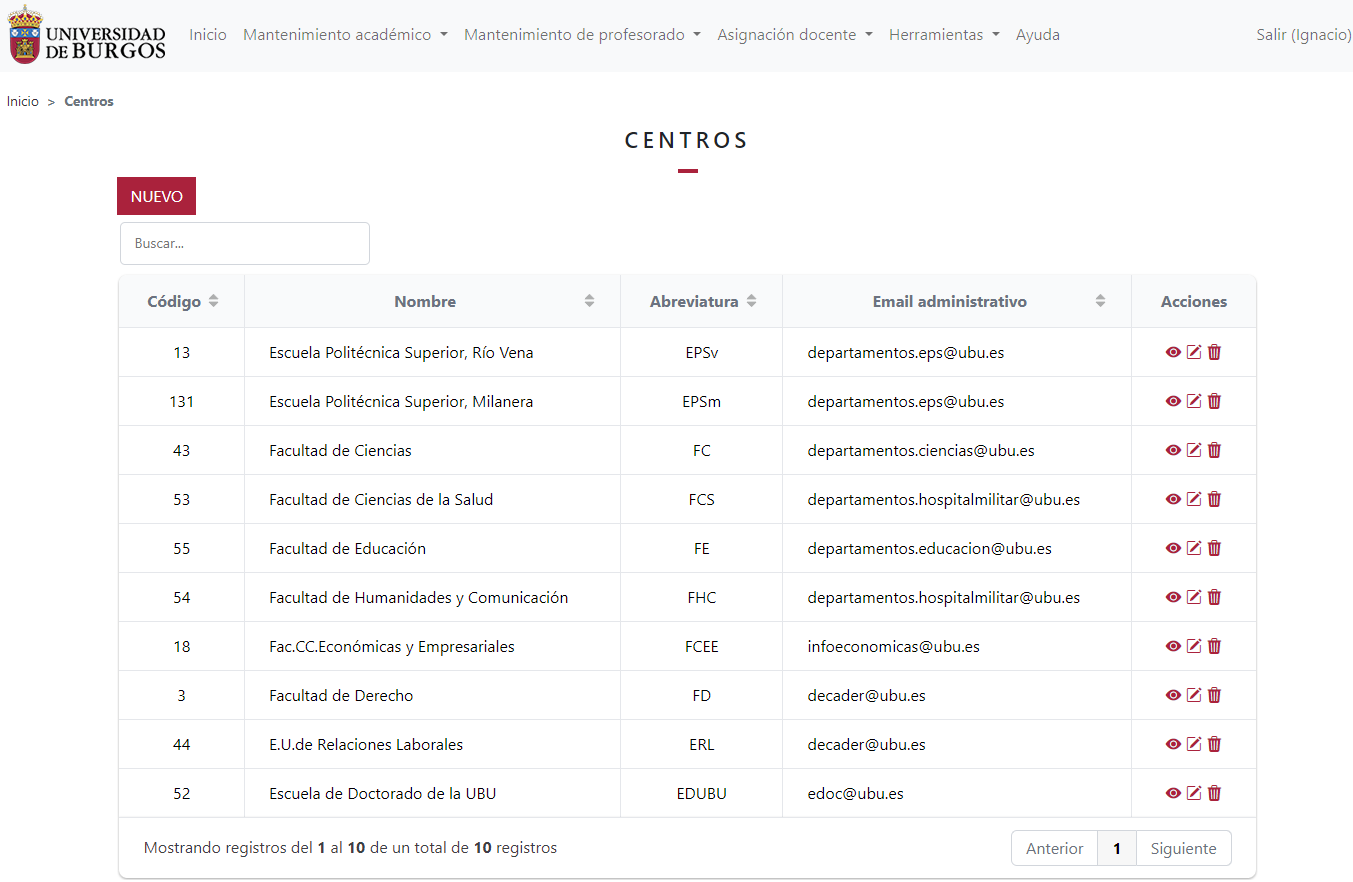
\includegraphics[width=\textwidth]{../img/Anexos/Manual usuario/centros.png}
	\caption{Página principal de centros}\label{pag:centros}
\end{figure}

\begin{figure}
	\centering
	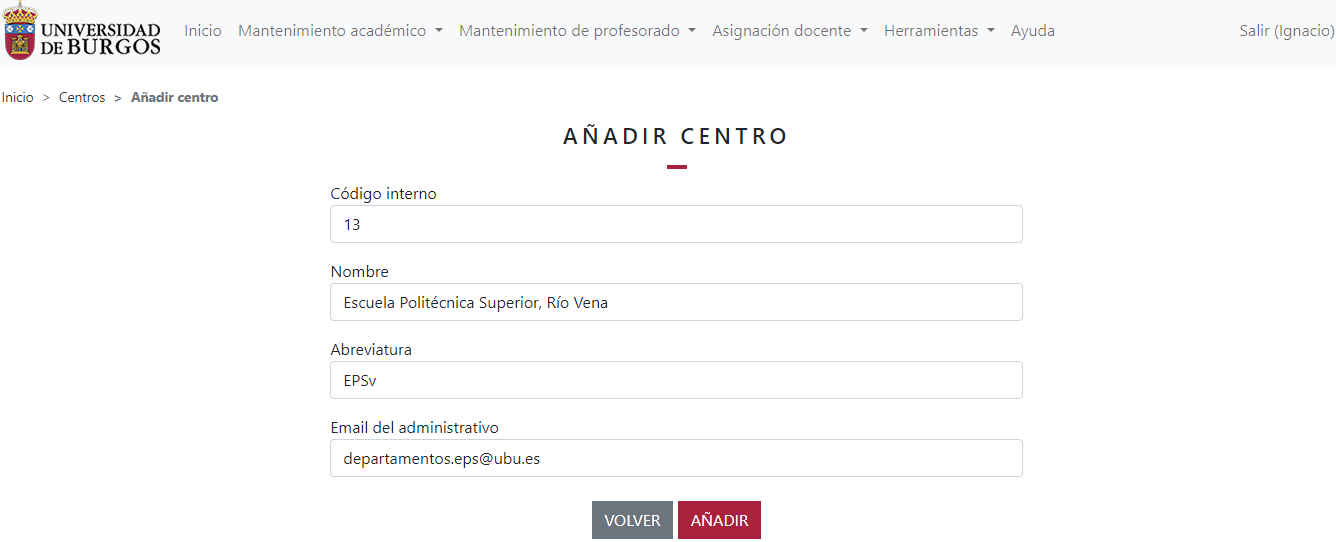
\includegraphics[width=\textwidth]{../img/Anexos/Manual usuario/formCentro.png}
	\caption{Formulario de creación de centros}\label{pag:formCentro}
\end{figure}

Desde la página del formulario se deben rellenar los campos con los datos del nuevo centro y pulsar sobre el botón <<Añadir>>.
Esto provocará que el centro se almacene en la base de datos. 
La aplicación redirigirá al usuario a la página principal de centros (imagen~\ref{pag:centros}) mostrando un mensaje que indica la correcta creación del centro.

\subsubsection{Modificación de centros}
Desde la página principal de centros (imagen~\ref{pag:centros}), se debe pulsar, en la tabla, sobre el icono del lápiz del centro que se desea modificar.
Esta acción provocará la redirección a la página del formulario de modificación, que contendrá los datos del centro seleccionado (imagen~\ref{pag:formModCentro}).

Desde esta página se pueden modificar los campos deseados y, al finalizar, pulsar sobre el botón <<Modificar>>.
Esta acción producirá una redirección a la página principal de centros, mostrando un mensaje que indica la correcta modificación del centro.

\begin{figure}
	\centering
	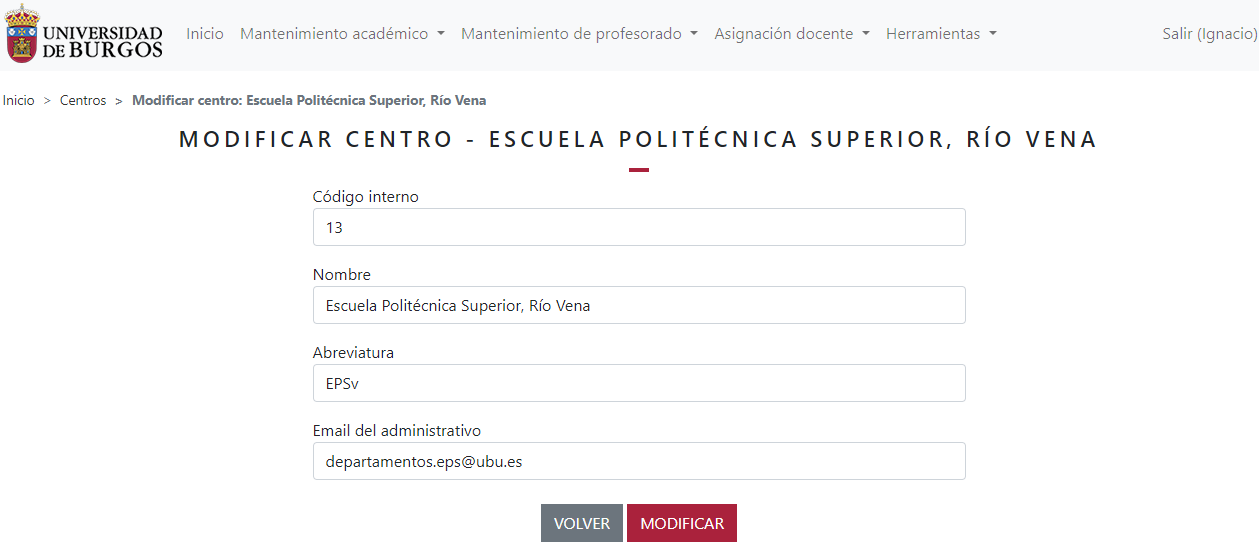
\includegraphics[width=\textwidth]{../img/Anexos/Manual usuario/formModCentro.png}
	\caption{Formulario de modificación de centros}\label{pag:formModCentro}
\end{figure}

\subsubsection{Eliminación de centros}
Desde la página principal de centros se puede eliminar un centro pulsando sobre el icono de la papelera del centro de la tabla que se desea eliminar.
Al hacer esto se mostrará la alerta de la imagen~\ref{pag:alertElCentro} y pulsando sobre el botón <<Aceptar>>, se realizará la petición de eliminación del centro.

Al hacer esto se mostrará un mensaje indicando la correcta eliminación o un mensaje indicando que no se ha podido realizar la eliminación en caso de que el centro tenga titulaciones asociadas.

\begin{figure}
	\centering
	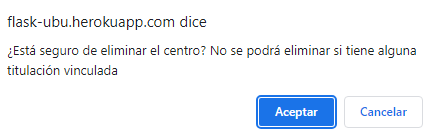
\includegraphics[width=\textwidth]{../img/Anexos/Manual usuario/alertElCentro.png}
	\caption{Alerta de eliminación de centros}\label{pag:alertElCentro}
\end{figure}

\subsubsection{Creación de titulaciones}
Pulsando sobre la opción del menú <<Titulaciones>> se accede a la vista principal de las titulaciones (ver imagen~\ref{pag:titulaciones}).

Para crear una nueva titulación se debe pulsar sobre el botón <<Nuevo>>.
Es importante tener en cuenta que para crear una titulación es necesario tener un centro creado previamente, ya que una titulación se vincula a un centro.

\begin{figure}
	\centering
	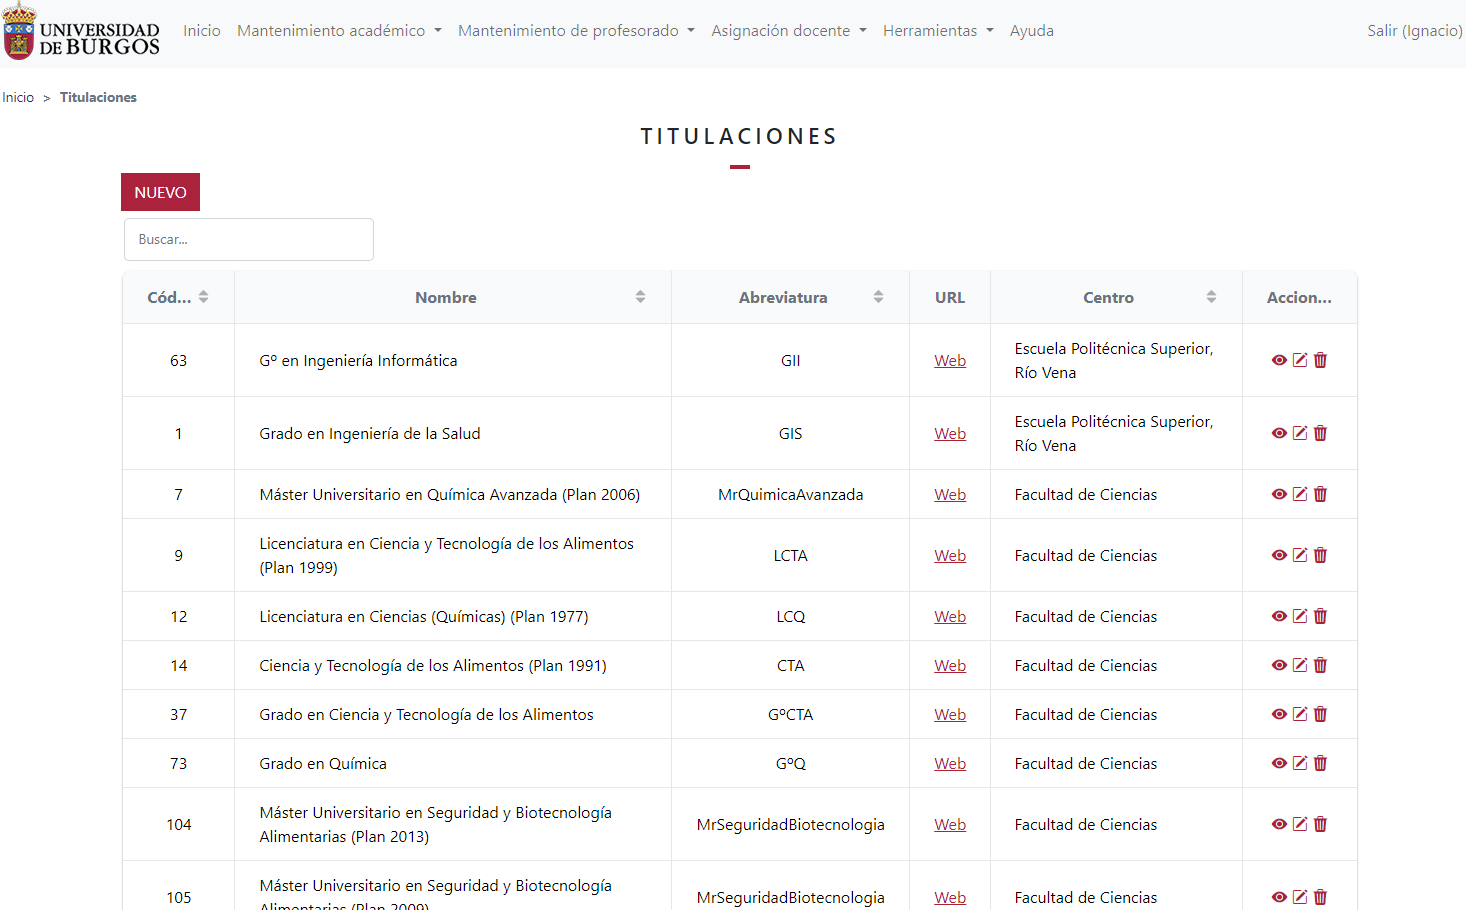
\includegraphics[width=\textwidth]{../img/Anexos/Manual usuario/titulaciones.png}
	\caption{Página principal de titulaciones}\label{pag:titulaciones}
\end{figure}

Al pulsar sobre el botón <<Nuevo>> se abre el formulario de creación de titulaciones.
Está página se puede ver en la imagen~\ref{pag:formTitulacion}.
En este formulario se deben introducir los datos de la titulación que se desea crear y, una vez se tengan los campos completados, pulsar sobre el botón <<Añadir>>.
Esta acción producirá una redirección a la página principal de titulaciones donde se podrá ver la titulación creada.
Además, se mostrará un mensaje indicando la creación de la titulación.

\begin{figure}
	\centering
	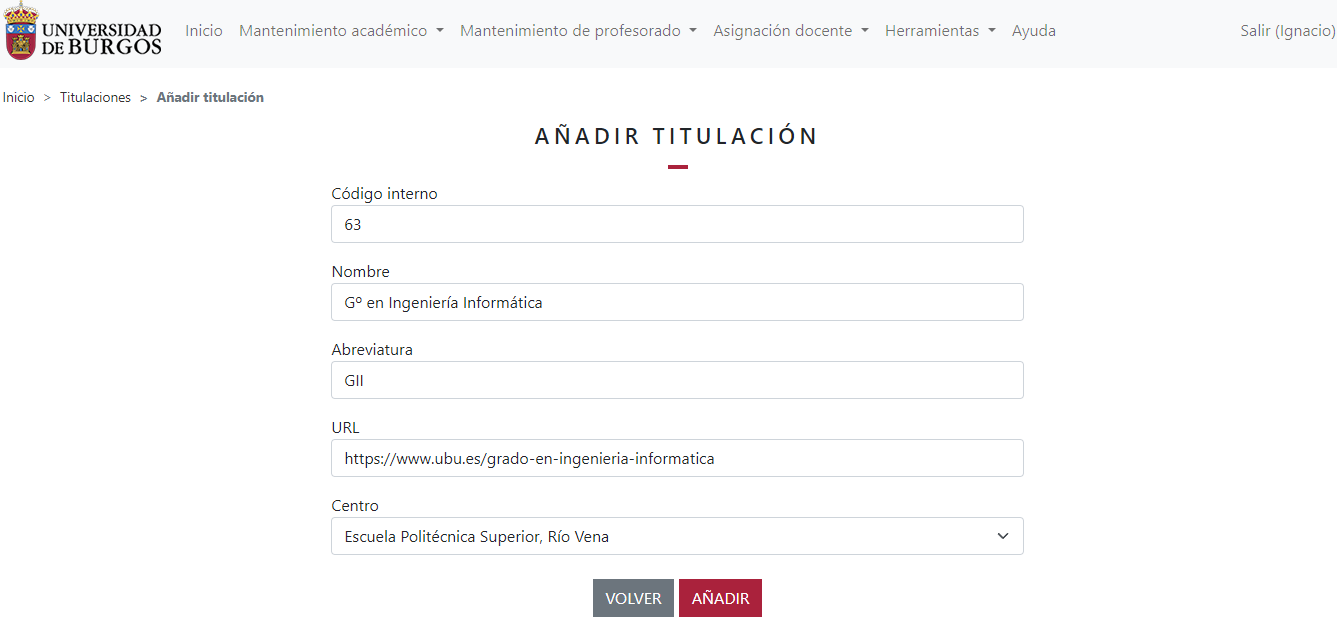
\includegraphics[width=\textwidth]{../img/Anexos/Manual usuario/formTitulacion.png}
	\caption{Formulario de creación de titulaciones}\label{pag:formTitulacion}
\end{figure}

\subsubsection{Modificación de titulaciones}
Para modificar una titulación, encontrándonos en la página principal de titulaciones (imagen~\ref{pag:titulaciones}), se debe pulsar sobre el icono de la lápiz de la titulación de la lista que se desea modificar.
Esto abrirá la página con el formulario de modificación de la titulación (ver imagen~\ref{pag:formModTitulacion}).

\begin{figure}
	\centering
	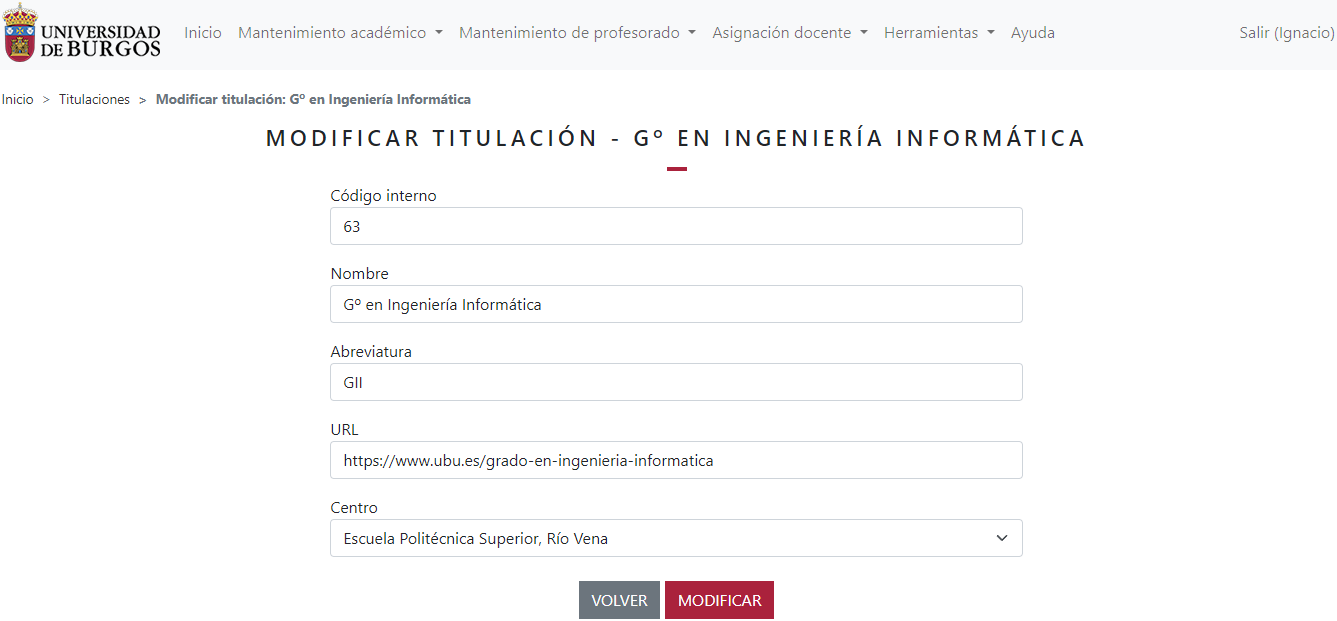
\includegraphics[width=\textwidth]{../img/Anexos/Manual usuario/formModTitulacion.png}
	\caption{Formulario de modificación de titulaciones}\label{pag:formModTitulacion}
\end{figure}

Desde este formulario se pueden modificar los campos deseados.
Una vez concluida la modificación se debe pulsar sobre el botón <<Modificar>>.
Esto plasmará los cambios en la base de datos y la web redirigirá al usuario a la página principal de titulaciones indicando mediante un mensaje la correcta modificación.

\subsubsection{Eliminación de titulaciones}
Desde la página principal de titulaciones (imagen~\ref{pag:titulaciones}), se debe pulsar sobre el icono de la papelera de la titulación que se desea eliminar.
Al realizar esta acción aparecerá en la pantalla la alerta de la imagen~\ref{pag:alertElTitulacion}. Si se pulsa sobre el botón <<Aceptar>> la titulación se eliminará de la base de datos si no tiene asignaturas asociadas, en caso contrario, no se podrá eliminar y aparecerá un mensaje de error mostrando esta información.

\begin{figure}
	\centering
	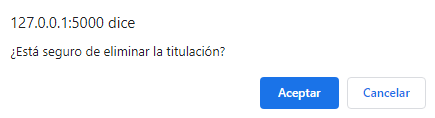
\includegraphics[width=\textwidth]{../img/Anexos/Manual usuario/alertElTitulacion.png}
	\caption{Alerta de eliminación de titulaciones}\label{pag:alertElTitulacion}
\end{figure}

\subsubsection{Creación de asignaturas}
Para añadir una nueva asignatura a la web, se debe pulsar sobre la opción del menú llamada <<Asignaturas>>.
Realizar esta acción redirige al usuario a la página principal de asignaturas (imagen~\ref{pag:asignaturas}).

Es importante tener en cuenta que previamente se debe haber creado la titulación a la que se quiere vincular la asignatura.

\begin{figure}
	\centering
	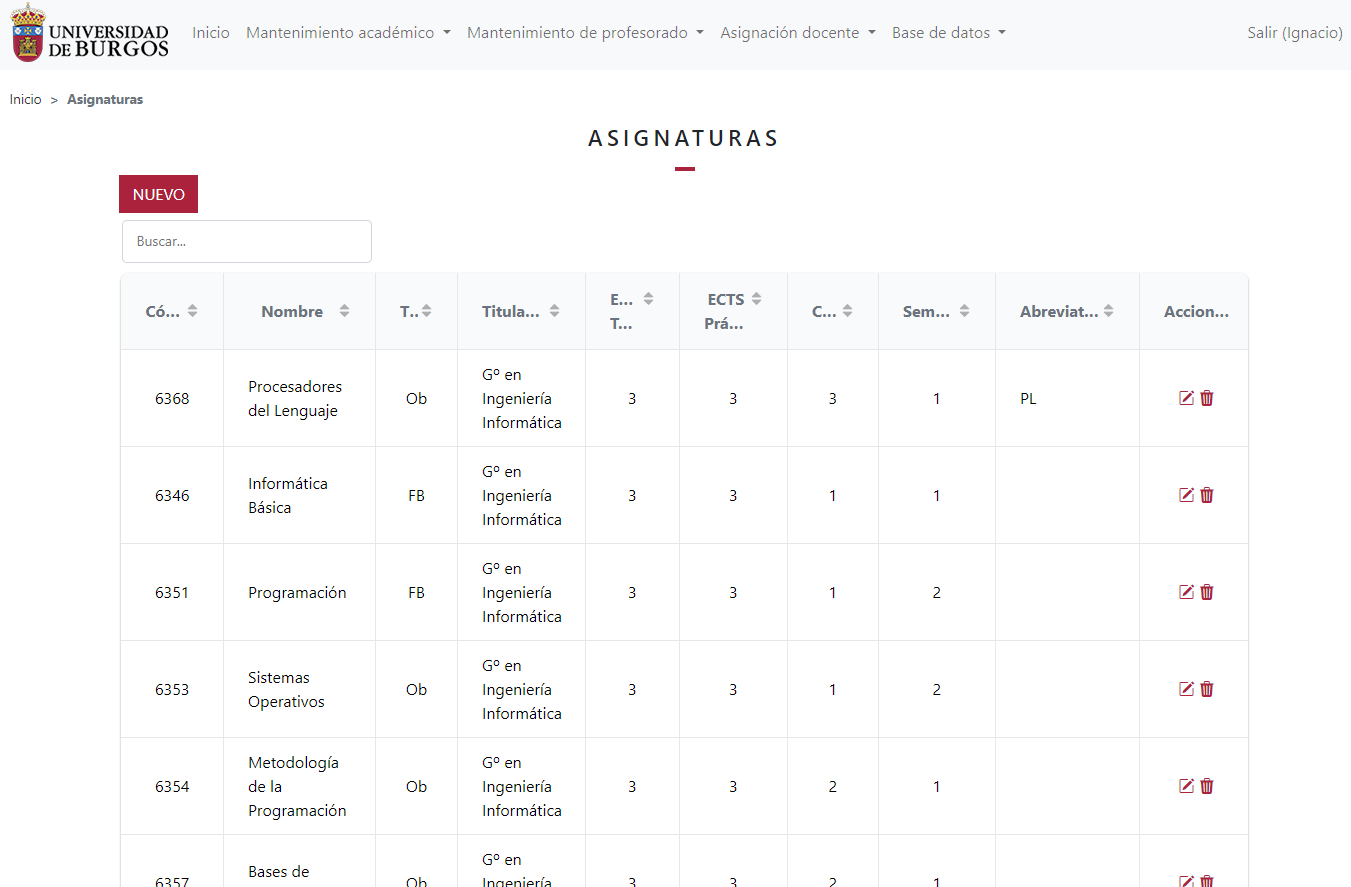
\includegraphics[width=\textwidth]{../img/Anexos/Manual usuario/asignaturas.png}
	\caption{Página principal de asignaturas}\label{pag:asignaturas}
\end{figure}

Una vez en la página principal de asignaturas se debe pulsar sobre el botón <<Nuevo>>, lo que abrirá el formulario de creación de asignaturas (ver imagen~\ref{pag:formAsignatura}).

Con los campos del formulario completados solo queda pulsar sobre el botón <<Añadir>> para almacenar la asignatura en la base de datos.
Tras realizar esta acción, se mostrará la página principal de asignaturas junto a un mensaje informando de la correcta creación de la asignatura.

\begin{figure}
	\centering
	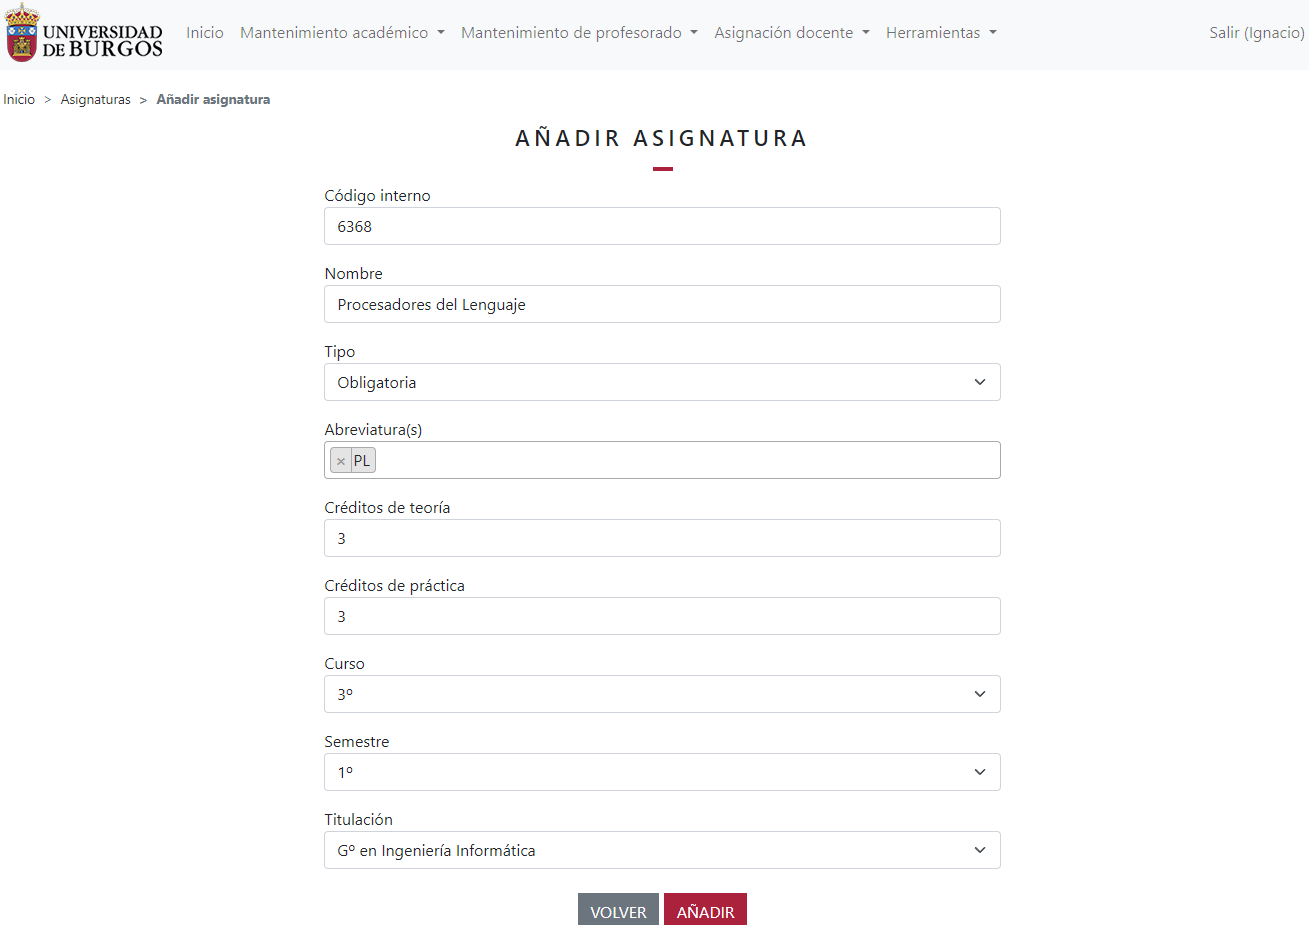
\includegraphics[width=\textwidth]{../img/Anexos/Manual usuario/formAsignatura.png}
	\caption{Formulario de creación de asignaturas}\label{pag:formAsignatura}
\end{figure}

\subsubsection{Modificación de asignaturas}
Para modificar una asignatura se debe pulsar sobre el icono del lápiz de la asignatura de la tabla que se desea modificar.
Esto abrirá el formulario de modificación de la asignatura con los campo rellenos con la información de la asignatura a editar (ver imagen~\ref{pag:formModAsignatura}).

En este momento se pueden editar los campos deseados y al finalizar, se debe pulsar sobre el botón <<Modificar>>.
Esto provocará el guardado de la información y una redirección a la página de asignaturas donde se mostrará un mensaje informativo sobre la modificación de la asignatura.

\begin{figure}
	\centering
	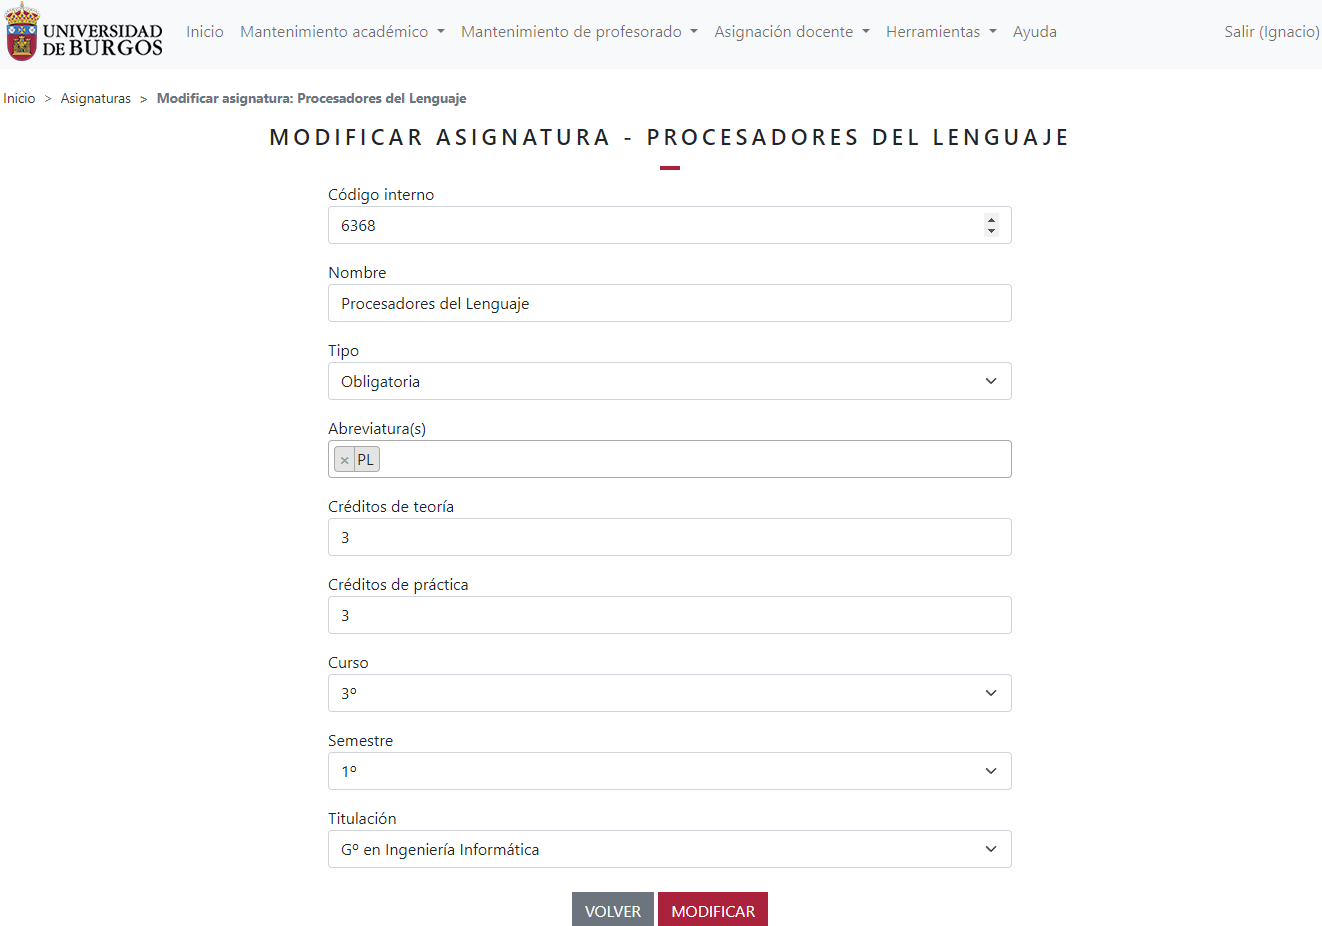
\includegraphics[width=\textwidth]{../img/Anexos/Manual usuario/formModAsignatura.png}
	\caption{Formulario de modificación de asignaturas}\label{pag:formModAsignatura}
\end{figure}

\subsubsection{Eliminación de asignaturas}
Si se desea eliminar una asignatura de la aplicación, se debe acceder a la página principal de asignaturas y, una vez aquí, pulsar sobre el icono de la papelera de la asignatura que se desea eliminar.

Al realizar la acción descrita, se abre una alerta de confirmación (ver imagen~\ref{pag:alertElAsignatura}).
Al pulsar sobre <<Aceptar>> la asignatura se elimina de la aplicación produciendo un borrado en cascada de sus relaciones con los cursos académicos creados.

\begin{figure}
	\centering
	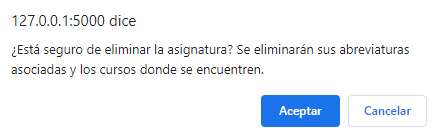
\includegraphics[width=.8\textwidth]{../img/Anexos/Manual usuario/alertElAsignatura.png}
	\caption{Alerta de eliminación de titulaciones}\label{pag:alertElAsignatura}
\end{figure}

\subsection{Mantenimiento de profesorado}
En esta sección se va a mostrar el manual de usuario sobre el mantenimiento de profesorado.
Esta parte de la aplicación incluye la creación, modificación y eliminación de los elementos que se pueden ver en la imagen~\ref{pag:menuManProf}.

\begin{figure}
	\centering
	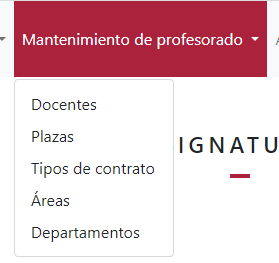
\includegraphics[width=.5\textwidth]{../img/Anexos/Manual usuario/menu man prof.png}
	\caption{Menú: Mantenimiento de profesorado}\label{pag:menuManProf}
\end{figure}

\subsubsection{Creación de docentes}
Para crear un nuevo docente, necesario para obtener acceso a la aplicación, se debe pulsar sobre la opción del menú llamada <<Docentes>>.
Esto abrirá la página principal de docentes (ver imagen~\ref{pag:docentes}).

\begin{figure}
	\centering
	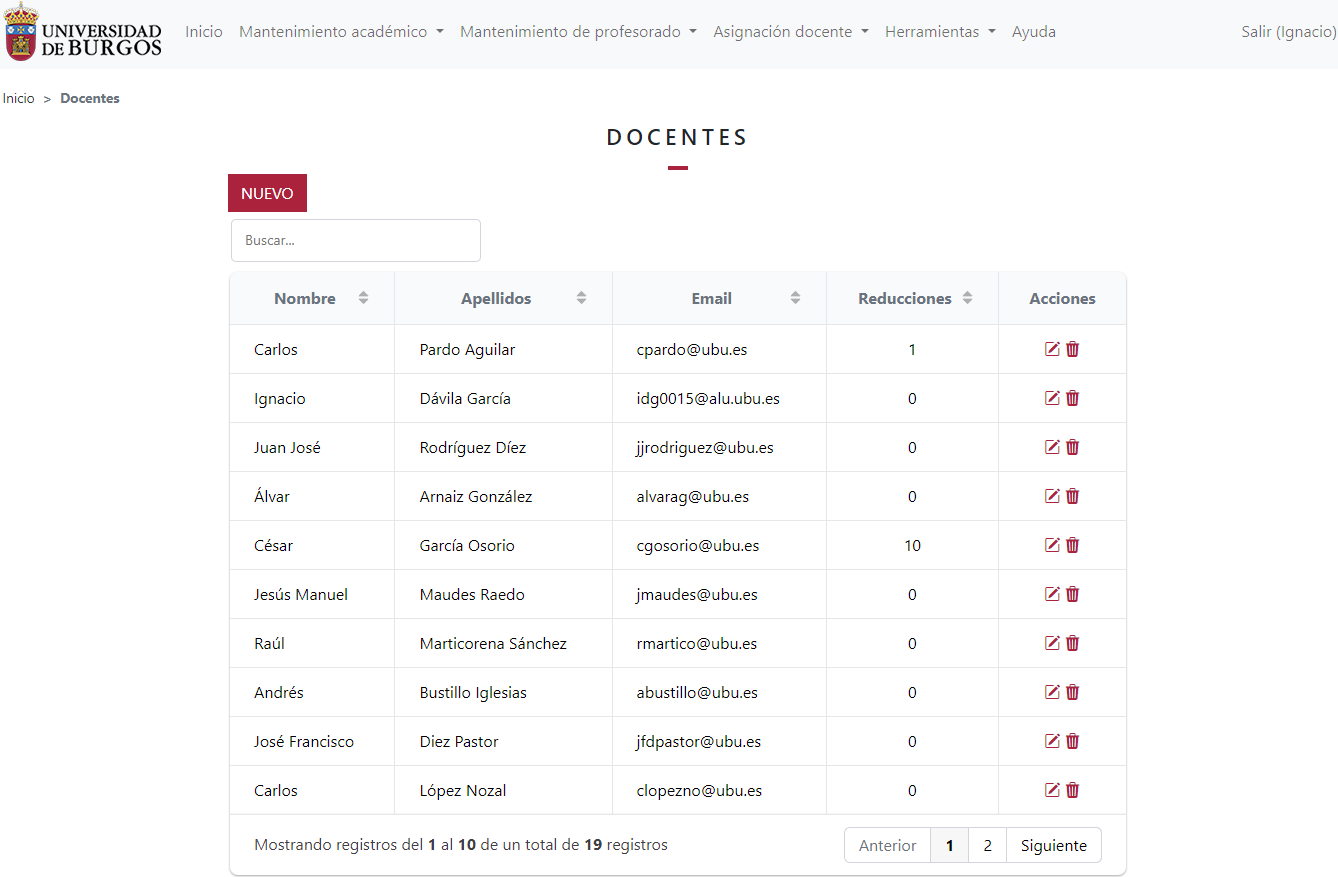
\includegraphics[width=\textwidth]{../img/Anexos/Manual usuario/docentes.png}
	\caption{Página principal de docentes}\label{pag:docentes}
\end{figure}

Desde esta página se debe pulsar sobre el botón <<Nuevo>>, lo que abrirá el formulario de creación de docentes (imagen~\ref{pag:formDocente}).

Una vez en la página del formulario, se deben rellenar los campos con los datos del docente que se desea añadir.
Es importante tener en cuenta que desde aquí se indican los permisos que tendrá el docente.
Si se le conceden permisos de modificación tendrá acceso a todas las funcionalidades descritas en este manual, mientras que si se le dan únicamente permisos de consulta, solo tendrá permiso para visualizar la información que administra la aplicación web.
Por último, en caso de no indicar ningún tipo de permiso, el usuario no tendrá acceso a la aplicación, aunque este dado de alta en el Moodle de la universidad.

\begin{figure}
	\centering
	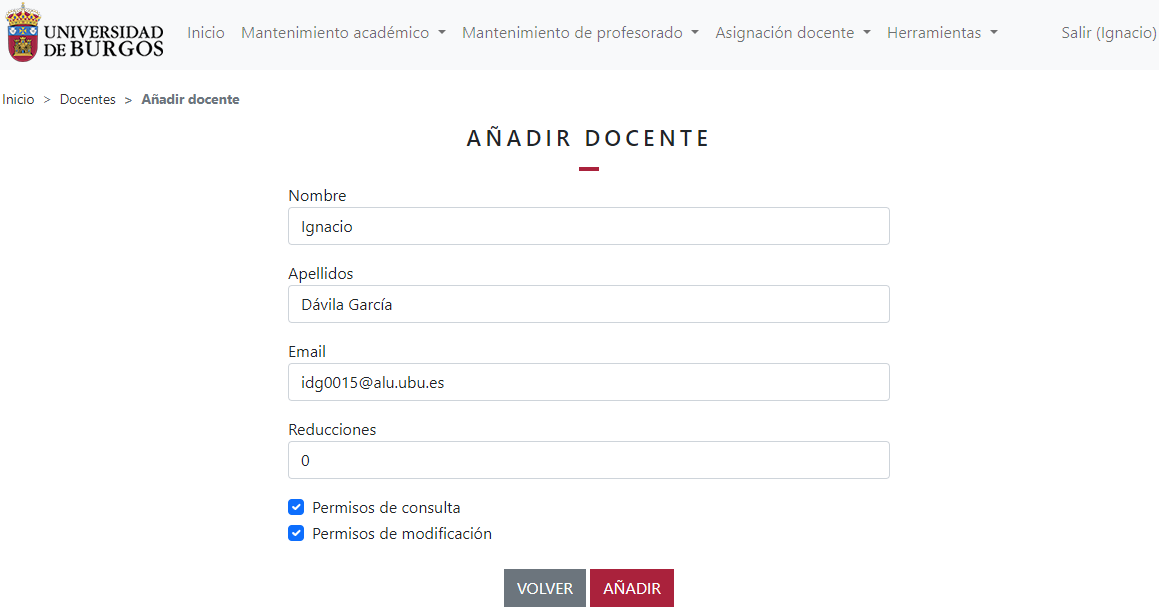
\includegraphics[width=\textwidth]{../img/Anexos/Manual usuario/formDocente.png}
	\caption{Formulario de creación de docentes}\label{pag:formDocente}
\end{figure}

\subsubsection{Modificación de docentes}
Para realizar la modificación de los datos de un docente se debe ir a la página principal de docentes (imagen~\ref{pag:docentes}).

Desde esta ventana se debe pulsar sobre el icono del lápiz del registro de la tabla correspondiente al docente que se desea modificar.
Esta acción producirá la redirección a la página del formulario de modificación del docente seleccionado, que se puede ver en la imagen~\ref{pag:formModDocente}.

\begin{figure}
	\centering
	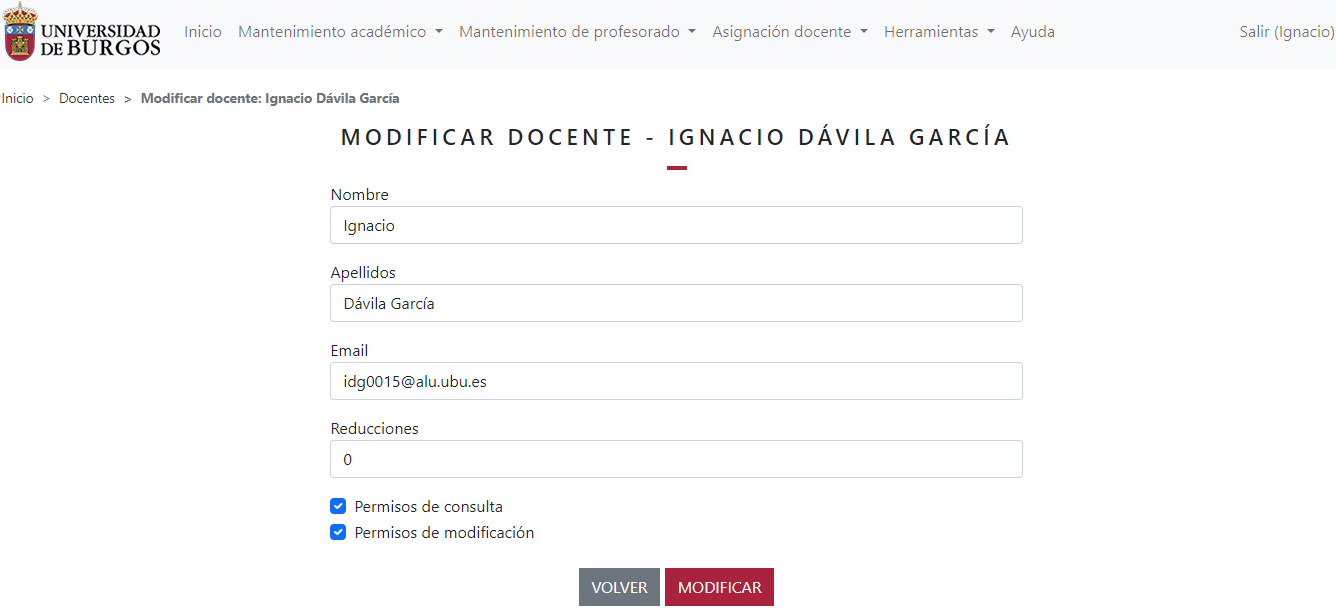
\includegraphics[width=\textwidth]{../img/Anexos/Manual usuario/formModDocente.png}
	\caption{Formulario de modificación de docentes}\label{pag:formModDocente}
\end{figure}

Una vez se hayan realizado los cambios deseados en los datos se debe pulsar sobre el botón de <<Modificar>>, lo que provocará la modificación en la base de datos de los datos y la redirección a la página principal de docentes donde se mostrará un mensaje indicando la correcta modificación.

\subsubsection{Eliminación de docentes}
Si se desea dar de baja de la base de datos a un docente se debe ir a la página principal de docentes donde se muestra una tabla con todos los que se encuentran dados de alta.
En esta tabla se debe buscar el docente a eliminar y pulsar sobre el icono de la papelera de la fila correspondiente al docente.

Tras realizar esta acción se abrirá una alerta de confirmación acerca de eliminar el docente.
Si se pulsa sobre <<Aceptar>> el docente desaparecerá de la base de datos y se podrá ver un mensaje indicando la correcta eliminación.

\subsubsection{Creación de plazas}
La creación de plazas se realiza accediendo a la página principal de plazas (imagen~\ref{pag:plazas}) al pulsar sobre la opción del menú <<Plazas>>.

\begin{figure}
	\centering
	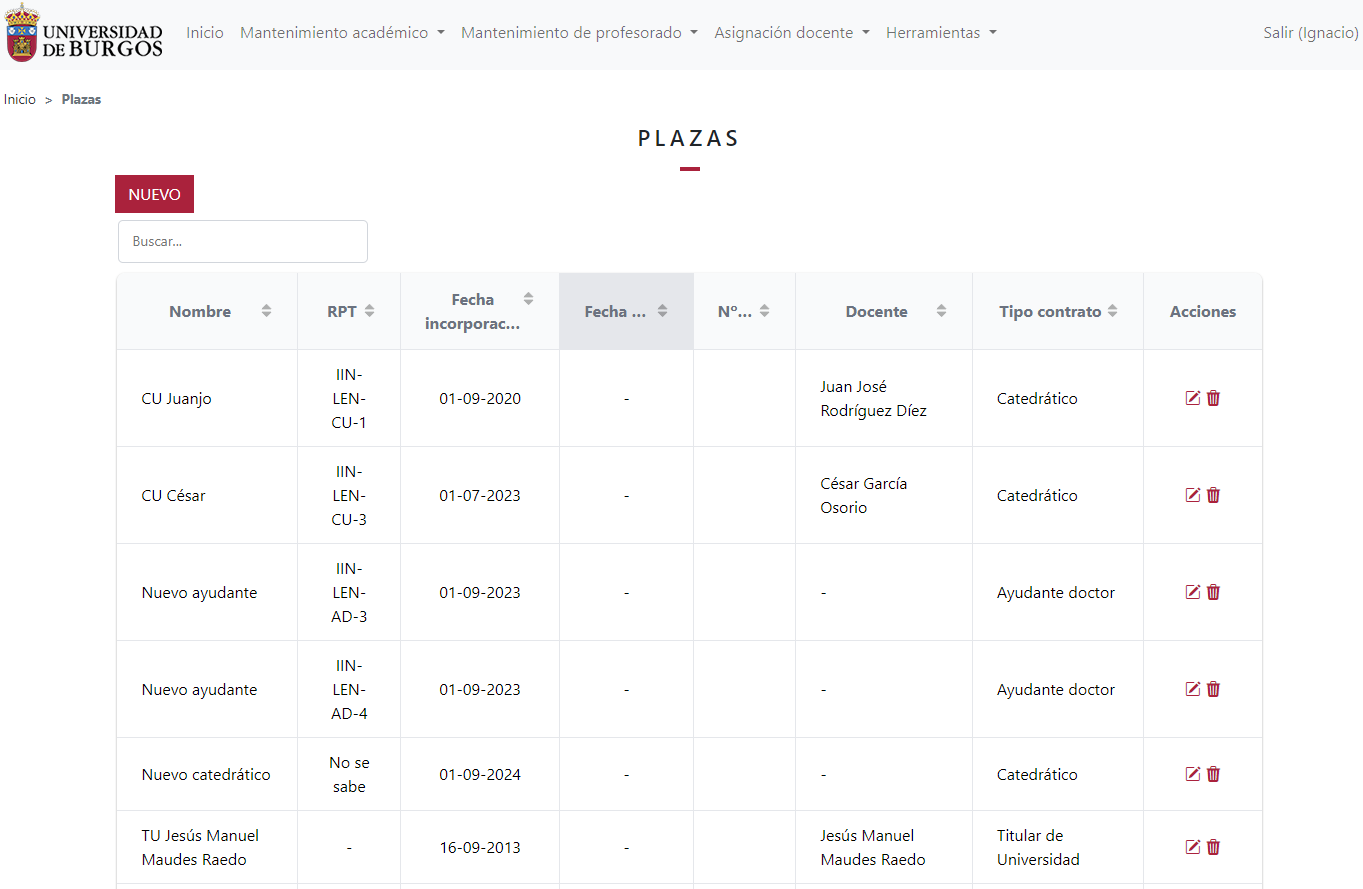
\includegraphics[width=\textwidth]{../img/Anexos/Manual usuario/plazas.png}
	\caption{Página principal de plazas}\label{pag:plazas}
\end{figure}

Desde esta ventana se debe pulsar sobre el botón <<Nuevo>>, lo que abrirá la página que contiene el formulario de creación de plazas (ver imagen~\ref{pag:formPlaza}).

\begin{figure}
	\centering
	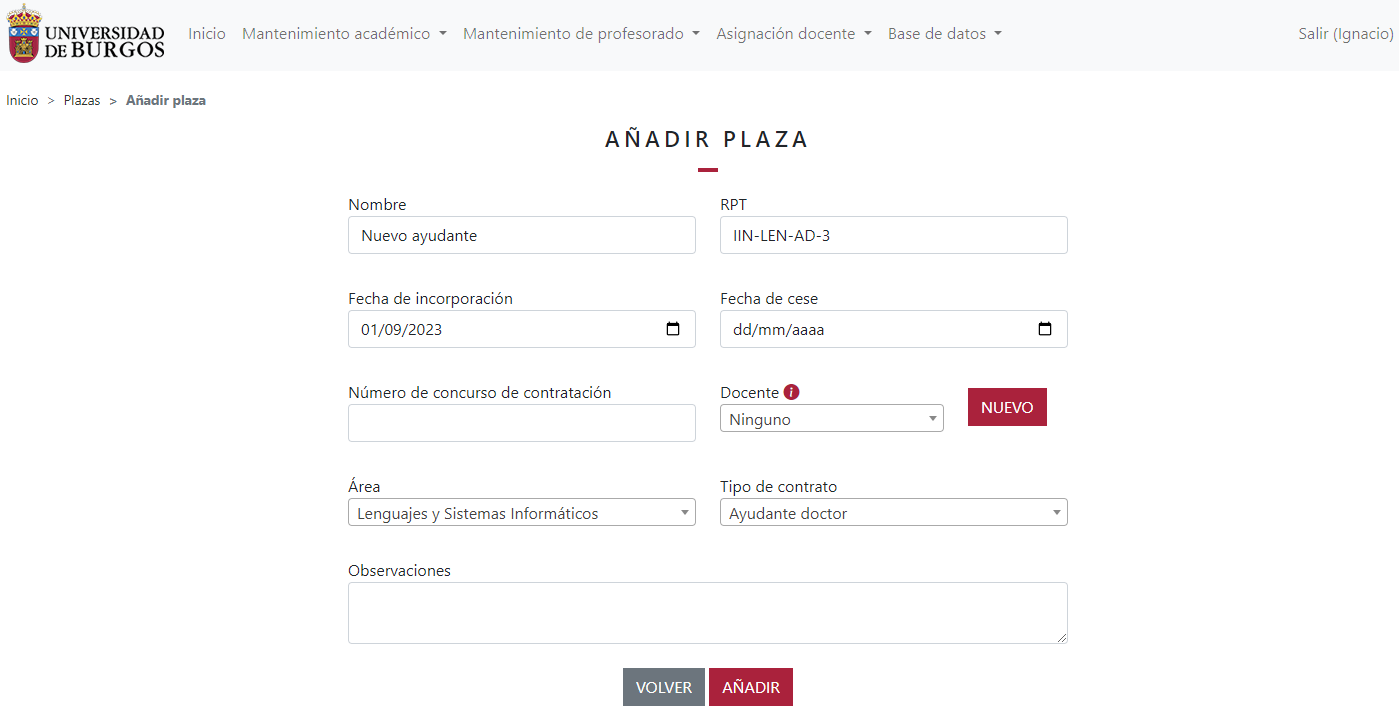
\includegraphics[width=\textwidth]{../img/Anexos/Manual usuario/formPlaza.png}
	\caption{Formulario de modificación de plazas}\label{pag:formPlaza}
\end{figure}

Desde está página se pueden completar los campos del formulario con los datos de la plaza que se desea dar de alta. 
Además, en caso de querer crear un docente en el mismo momento de creación de la plaza, se puede pulsar sobre el botón <<Nuevo>> del campo llamado <<Docente>>.
Esto abrirá una ventana modal con el formulario de creación de docentes (imagen~\ref{pag:formDocente}) desde el que se podrá crear el docente que después podrá ser seleccionado desde el formulario de plazas.

Es importante tener en cuenta de que para crear una nueva plaza es necesario tener creada previamente el área a la que pertenecerá la plaza y el tipo de contrato que tendrá.

Cuando se tengan todos los campos obligatorios completados, se debe pulsar sobre el botón <<Añadir>>.
Tras esta acción la web redirigirá a la página principal de plazas mostrando un mensaje informando sobre la creación de la plaza.

\subsubsection{Modificación de plazas}
Para realizar la modificación de los datos de una plaza se debe acceder a la página principal de plazas (figura~\ref{pag:plazas}).

Una vez en esa página se debe pulsar sobre el icono del lápiz de la plaza que se desea modificar.
Esto abrirá la página que contiene el formulario de modificación de plazas (imagen~\ref{pag:formModPlaza}) con todos los datos de la plaza disponibles para ser editados.

Una vez se tengan los campos deseados editados, se debe pulsar sobre el botón <<Modificar>>.
De esta manera la información quedará actualizada y seremos redirigidos a la página principal de plazas, donde se podrán ver reflejados los cambios. 
También se mostrará un mensaje informando de la modificación de la plaza.

\begin{figure}
	\centering
	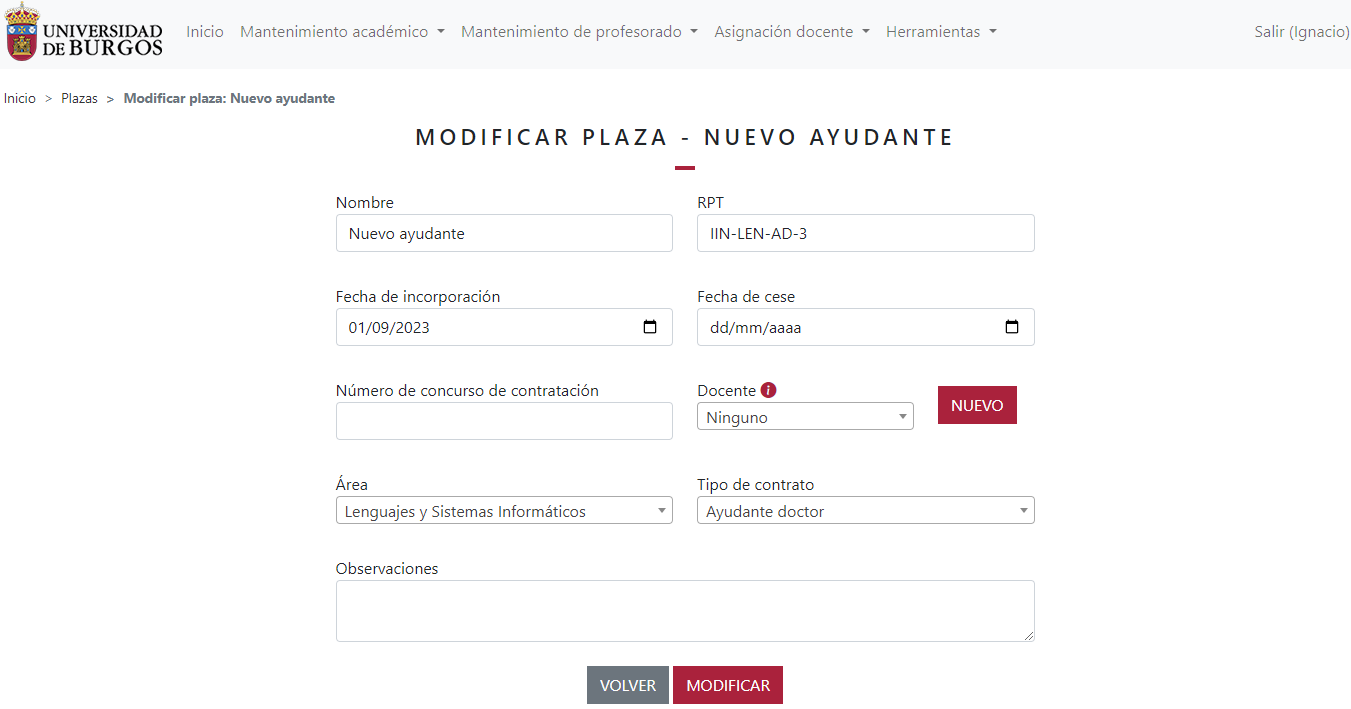
\includegraphics[width=\textwidth]{../img/Anexos/Manual usuario/formModPlaza.png}
	\caption{Formulario de modificación de plazas}\label{pag:formModPlaza}
\end{figure}

\subsubsection{Eliminación de plazas}
Si se desea eliminar una plaza que se encuentra en la aplicación web, se debe ir a la página principal de plazas y, desde esta página, se debe pulsar en el icono de la papelera de la plaza del listado que se desea eliminar.
Esta acción provocará la apertura de una alerta de confirmación como la de la figura~\ref{pag:alertElPlaza} en la que se informa de que, en caso de eliminar la plaza, se eliminarán con ella las posibles relaciones que tenga con grupos de las asignaturas del curso académico correspondiente.

Si se pulsa en <<Aceptar>> la plaza y sus vinculaciones quedan eliminadas, y se mostrará un mensaje informando de la eliminación.

\begin{figure}
	\centering
	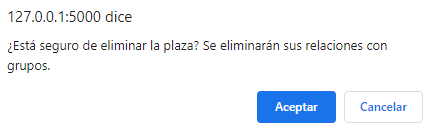
\includegraphics[width=.5\textwidth]{../img/Anexos/Manual usuario/alertElPlaza.png}
	\caption{Alerta de eliminación de plaza}\label{pag:alertElPlaza}
\end{figure}

\subsubsection{Creación de tipos de contrato}
En este apartado se va a mostrar la información necesaria para poder crear un nuevo tipo de contrato.

Para comenzar se debe pulsar la opción del menú <<Tipos de contrato>> que se encuentra dentro de <<Mantenimiento de profesorado>>.
Al realizar esta acción la web nos mostrará la pantalla principal de los contratos (ver imagen~\ref{pag:contratos}).

\begin{figure}
	\centering
	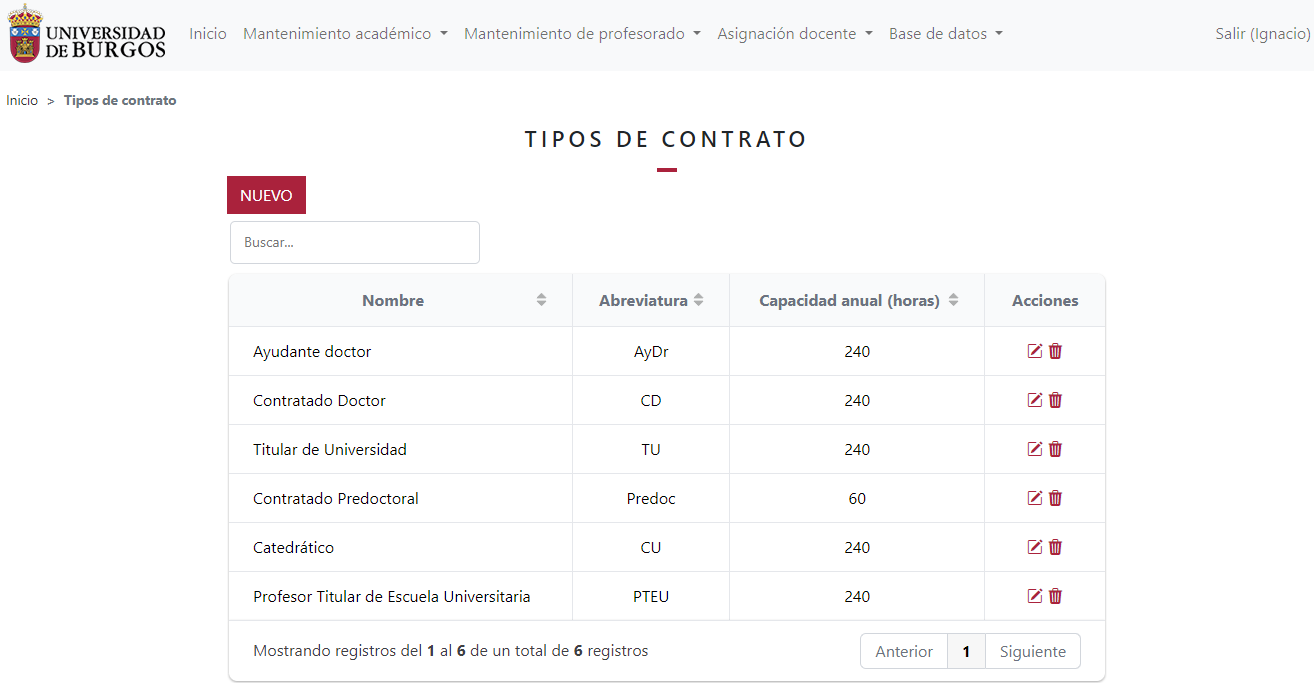
\includegraphics[width=\textwidth]{../img/Anexos/Manual usuario/contratos.png}
	\caption{Página principal de tipos de contrato}\label{pag:contratos}
\end{figure}

Para crear el nuevo tipo de contrato se debe pulsar sobre el botón <<Nuevo>> que aparece en la página, encima de la tabla.
Esto hará una redirección al formulario de creación de tipos de contrato (imagen~\ref{pag:formContrato}).

En este formulario se deben ingresar los datos del nuevo tipo de contrato que se desea crear.
Una vez se tenga el formulario completo hay que pulsar sobre el botón <<Añadir>>.
Al realizar esta acción, la página web nos redirigirá a la página principal de tipos de contrato.
Además, aparecerá un mensaje informando acerca de la creación del tipo de contrato.

\begin{figure}
	\centering
	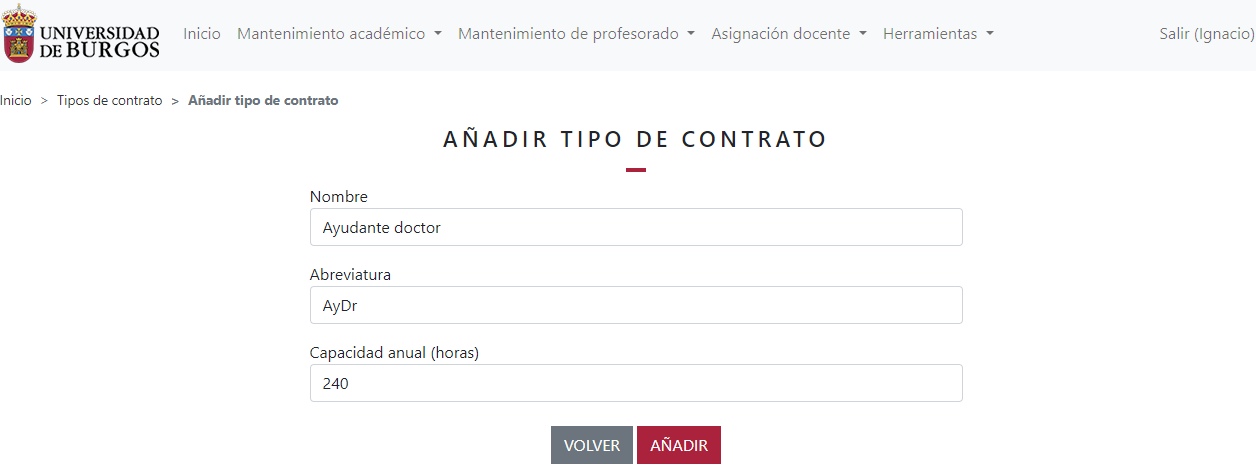
\includegraphics[width=\textwidth]{../img/Anexos/Manual usuario/formContrato.png}
	\caption{Formulario de creación de tipos de contrato}\label{pag:formContrato}
\end{figure}

\subsubsection{Modificación de tipos de contrato}
Si se desea modificar la información de un tipo de contrato se debe acceder a la página principal de tipos de contrato.

Desde esta página se debe buscar el tipo de contrato a modificar en la tabla y se debe pulsar sobre el icono del lápiz de la columna <<Acciones>>.
Al hacer esto la web nos llevará al formulario de modificación del tipo de contrato (ver imagen~\ref{pag:formModContrato}), que tendrá todos los campos rellenos con la información aportada a la hora de haberlo creado.

Cuando se hayan modificado los campos deseados se debe pulsar sobre el botón <<Modificar>>.
De esta manera la información quedará actualizada y volveremos a la página principal donde se mostrará un mensaje con información sobre la modificación realizada.

\begin{figure}
	\centering
	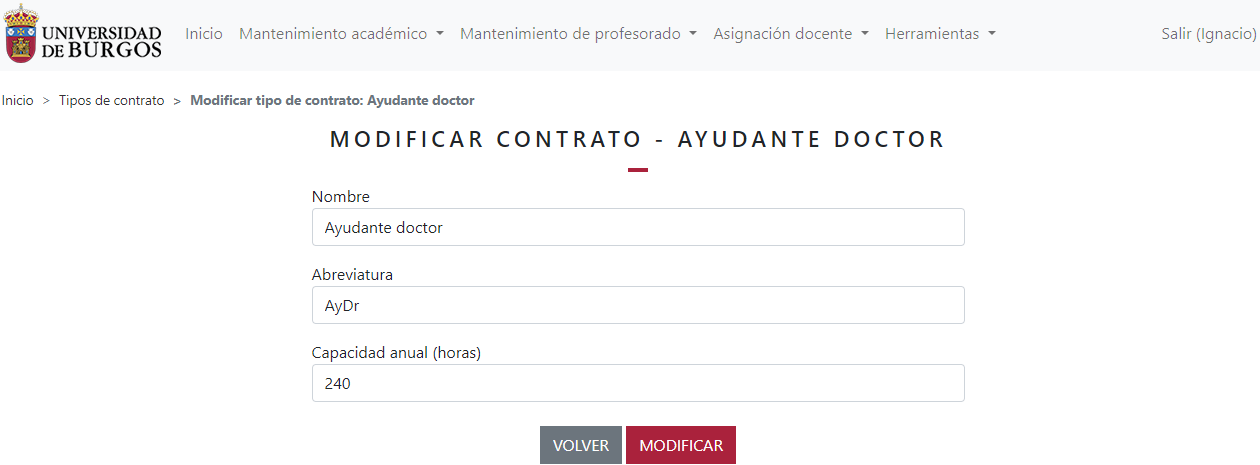
\includegraphics[width=\textwidth]{../img/Anexos/Manual usuario/formModContrato.png}
	\caption{Formulario de modificación de tipos de contrato}\label{pag:formModContrato}
\end{figure}

\subsubsection{Eliminación de tipos de contrato}
En este apartado se van a indicar los pasos necesarios para realizar la eliminación de un tipo de contrato.

En primer lugar debemos dirigirnos a la página principal de tipos de contrato.
En esta página se encuentra una tabla que contiene todos los tipos de contrato creados.

Para eliminar un tipo de contrato se debe pulsar sobre el icono de la papelera de la fila correspondiente a ese tipo de contrato.
Al realizar esta acción aparecerá la alerta de la imagen~\ref{pag:alertElContrato}, que sirve confirmar la eliminación del tipo de contrato.

Como se puede ver en el mensaje de la alerta de la imagen anterior, la eliminación de un tipo de contrato supone la eliminación de todas las plazas que utilicen ese tipo de contrato, lo que provocará una eliminación de todos los elementos que dependan de dichas plazas.

\begin{figure}
	\centering
	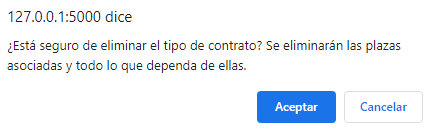
\includegraphics[width=.6\textwidth]{../img/Anexos/Manual usuario/alertElContrato.png}
	\caption{Alerta de eliminación de tipo de contrato}\label{pag:alertElContrato}
\end{figure}


\subsubsection{Creación de áreas}
La creación de nuevas áreas se realiza desde la página principal de áreas.
Para acceder a esta página se debe pulsar sobre la opción del menú llamada <<Áreas>> que se encuentra dentro de la opción desplegable llamada <<Mantenimiento de profesorado>>.

Al acceder a la página principal de áreas (ver imagen~\ref{pag:areas}) se debe pulsar sobre el botón <<Nuevo>>, lo que nos dirigirá al formulario de creación de áreas (imagen~\ref{pag:formArea}).

\begin{figure}
	\centering
	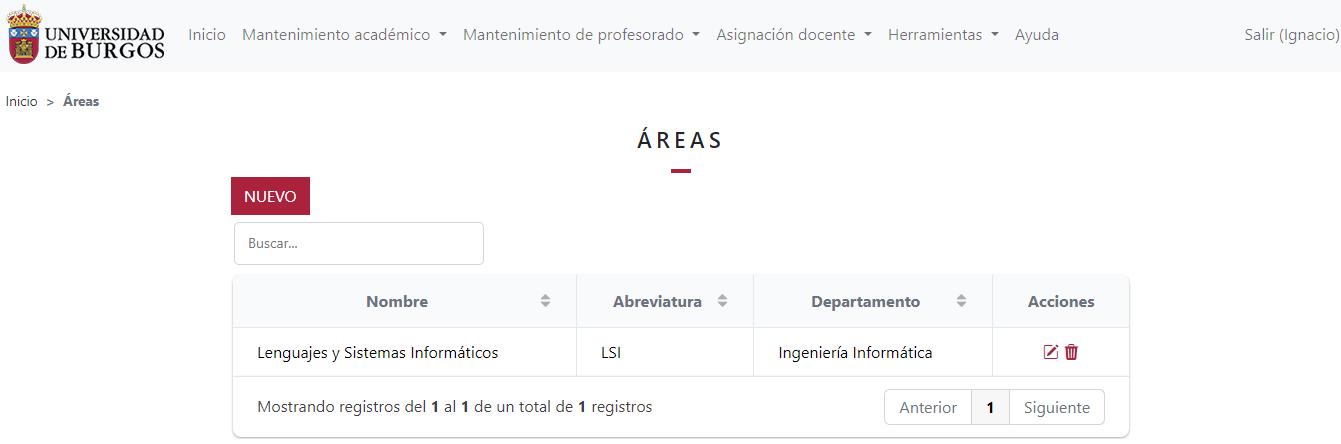
\includegraphics[width=\textwidth]{../img/Anexos/Manual usuario/areas.png}
	\caption{Página principal de áreas}\label{pag:areas}
\end{figure}

\begin{figure}
	\centering
	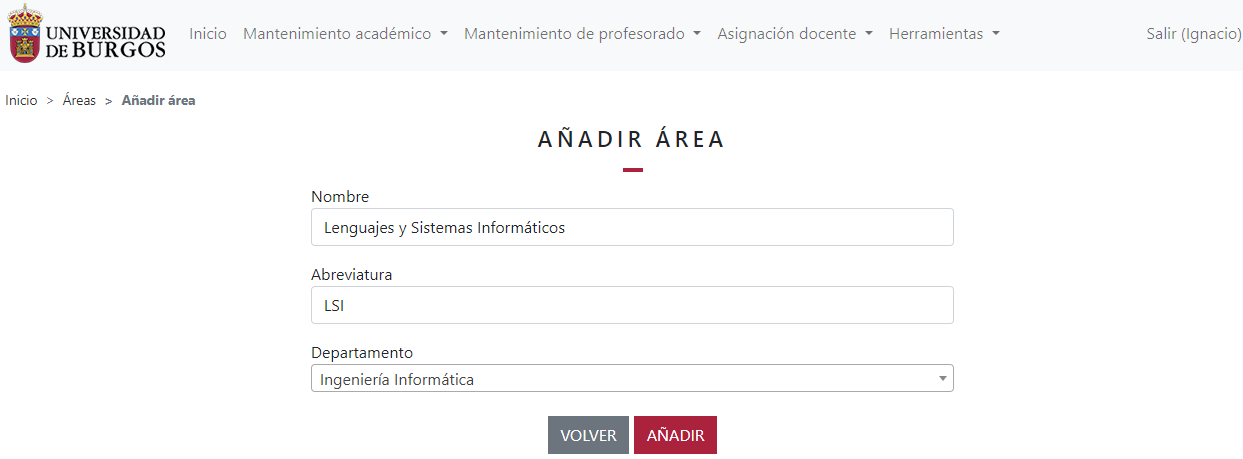
\includegraphics[width=\textwidth]{../img/Anexos/Manual usuario/formArea.png}
	\caption{Formulario de creación de áreas}\label{pag:formArea}
\end{figure}

En este formulario se deben ingresar los datos del área que se desea crear y, una vez este completo, pulsar sobre el botón <<Añadir>>.

Una vez realizado este proceso el área se habrá almacenado en la base de datos y la web nos redirigirá a la página principal de áreas mostrando un mensaje con información sobre la creación.

\subsubsection{Modificación de áreas}
Si necesitamos modificar la información de un área debemos dirigirnos a la página principal de áreas y pulsar sobre el icono del lápiz del área que se desea actualizar.
Pulsar sobre el icono hará que la web nos redireccione a la página que contiene el formulario de modificación del área (imagen~\ref{pag:formModArea}).

\begin{figure}
	\centering
	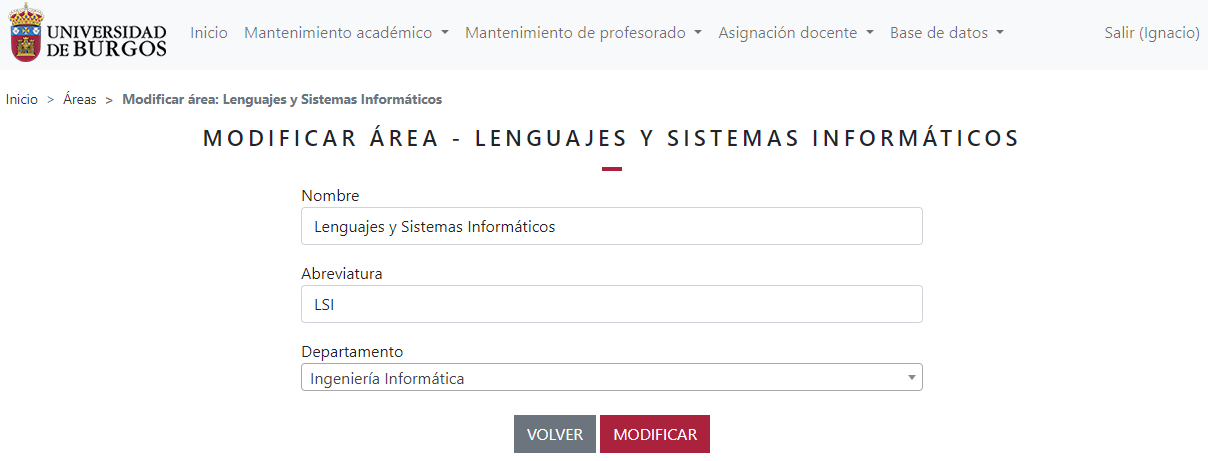
\includegraphics[width=\textwidth]{../img/Anexos/Manual usuario/formModArea.png}
	\caption{Formulario de modificación de áreas}\label{pag:formModArea}
\end{figure}

Desde esta página se pueden editar los campos deseados y, una vez finalice la modificación, pulsar sobre el botón <<Modificar>> para hacer efectivos los cambios.

\subsubsection{Eliminación de áreas}
Para eliminar un área debemos pulsar sobre la opción del menú <<Áreas>> y, una vez en la página principal de áreas, pulsar sobre el icono de la papelera del área que se desea eliminar.

Al realizar esta acción se abrirá una alerta para confirmar la eliminación como la de la imagen~\ref{pag:alertElArea}.

Si se pulsa sobre <<Aceptar>>, se eliminará el área produciendo un borrado en cascada de las plazas dependientes y, por lo tanto, de todo lo relacionado con las plazas.

\begin{figure}
	\centering
	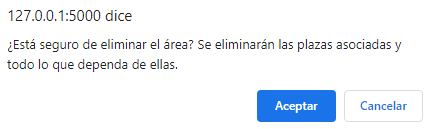
\includegraphics[width=.6\textwidth]{../img/Anexos/Manual usuario/alertElArea.png}
	\caption{Alerta de eliminación de área}\label{pag:alertElArea}
\end{figure}


\subsubsection{Creación de departamentos}
Ante la necesidad de crear un nuevo departamento, debemos desplazarnos al menú de la aplicación web y pulsar sobre la opción llamada <<Departamentos>>. 
Esta acción provocará que se muestre en la pantalla la página principal de los departamentos (ver imagen~\ref{pag:departamentos}), donde se puede ver una tabla con todos los departamentos creados.

Para crear un nuevo departamento se debe pulsar sobre el botón <<Nuevo>>.
Esta acción abrirá una nueva página con el formulario de creación de departamentos (imagen~\ref{pag:formDepartamento}).

Tras rellenar el formulario con los datos del departamento que se desea dar de alta, se debe pulsar sobre el botón <<Añadir>>.
De esta forma el departamento quedará creado y el usuario será redirigido a la página principal de departamentos donde se mostrará un mensaje informativo acerca de la creación realizada.

\begin{figure}
	\centering
	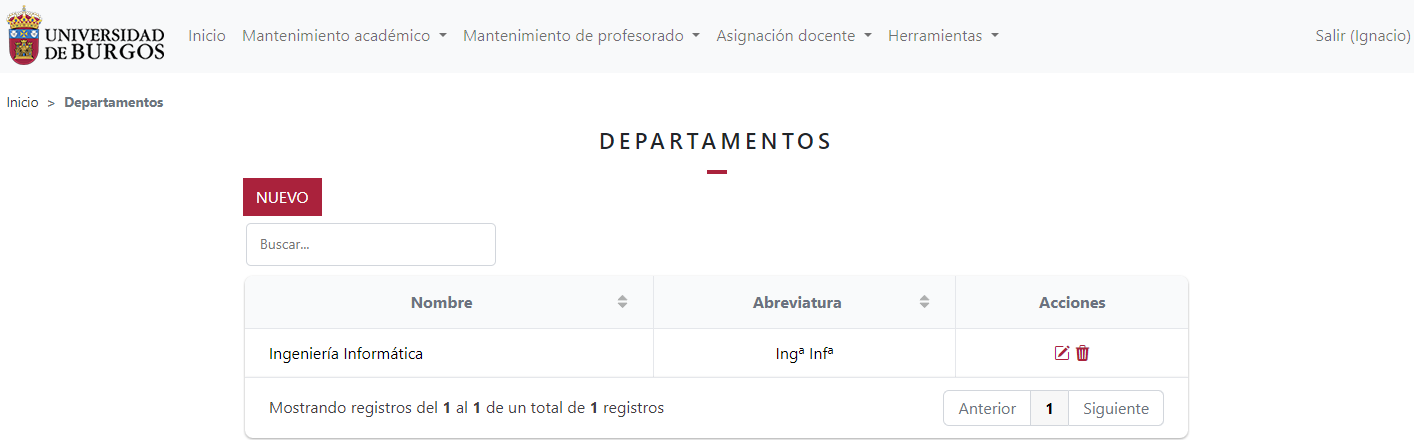
\includegraphics[width=\textwidth]{../img/Anexos/Manual usuario/departamentos.png}
	\caption{Página principal de departamentos}\label{pag:departamentos}
\end{figure}

\begin{figure}
	\centering
	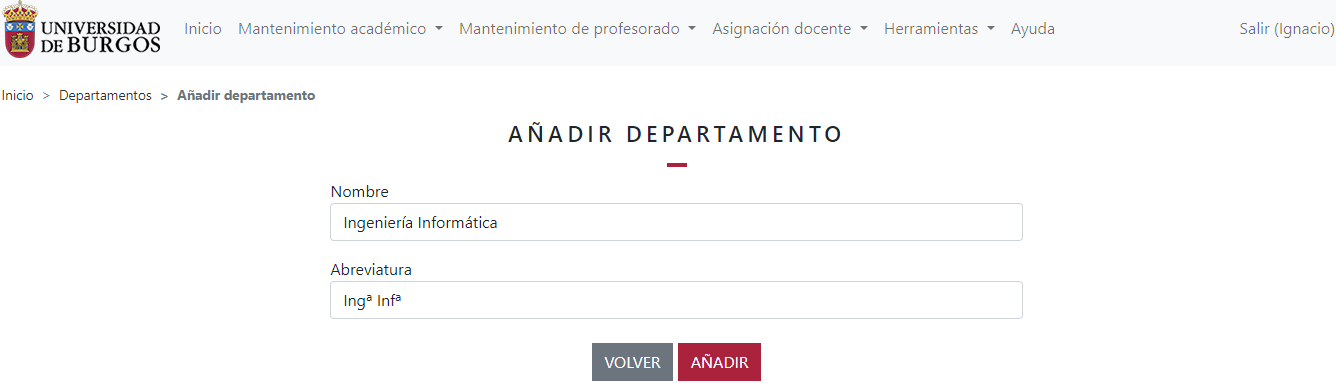
\includegraphics[width=\textwidth]{../img/Anexos/Manual usuario/formDepartamento.png}
	\caption{Formulario de creación de departamentos}\label{pag:formDepartamento}
\end{figure}

\subsubsection{Modificación de departamentos}
Para modificar los datos de un departamento debemos ir a la página principal de departamentos y, una vez ahí, pulsar sobre el icono del lápiz del departamento que se desea actualizar.
Esta acción provocará la redirección al formulario de modificación del departamento que se puede ver en la image~\ref{pag:formModDepartamento}.

Tras modificar los campos deseados, se debe pulsar en el botón <<Modificar>> para hacer los cambios efectivos.
De esta manera, se volverá a la página principal de departamentos donde se verá un mensaje indicando la modificación del departamento.

\begin{figure}
	\centering
	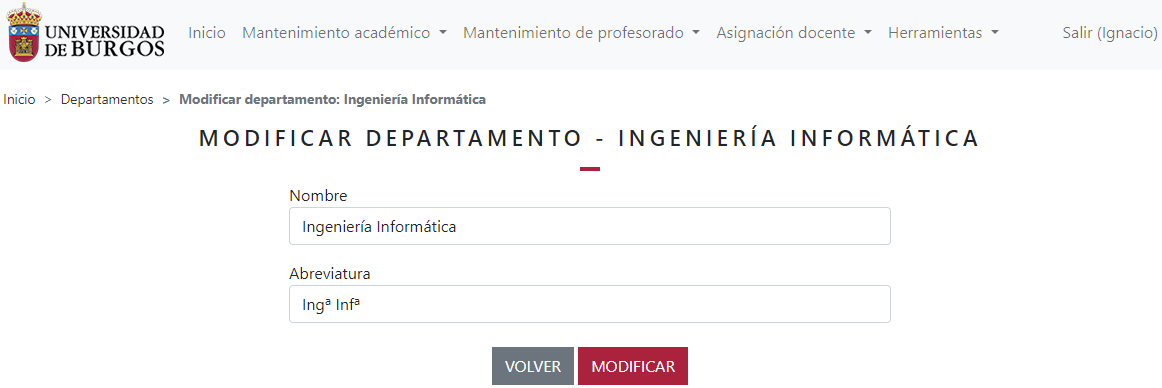
\includegraphics[width=\textwidth]{../img/Anexos/Manual usuario/formModDepartamento.png}
	\caption{Formulario de modificación de departamentos}\label{pag:formModDepartamento}
\end{figure}

\subsubsection{Eliminación de departamentos}
Si se desea dar de baja un departamento se debe ir a la página principal de departamentos y pulsar sobre el icono de la papelera del departamento que se desea eliminar.
Esta acción hará que se abra una alerta (imagen~\ref{pag:alertElDepartamento}) desde la que confirmar la eliminación.

Es importante tener en cuenta que la eliminación de un departamento supone eliminar todas las áreas que se encuentran vinculadas a este, y al borrar las áreas, se eliminará todo lo que se relacione o dependa de ellas.

\begin{figure}
	\centering
	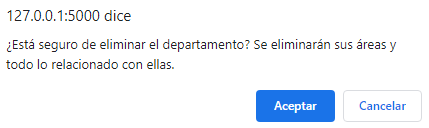
\includegraphics[width=.6\textwidth]{../img/Anexos/Manual usuario/alertElDepartamento.png}
	\caption{Alerta de eliminación de departamento}\label{pag:alertElDepartamento}
\end{figure}
